\documentclass[a4paper,12pt,abstracton,titlepage]{scrartcl}
\usepackage{scrpage2}
\usepackage[utf8]{inputenc}
\usepackage[T1]{fontenc}
\usepackage[top=2cm, bottom=2cm, left=2cm, right=2cm]{geometry}
\usepackage[affil-it]{authblk}
\usepackage{lipsum}
\usepackage[hidelinks]{hyperref}
\usepackage{graphicx}
\usepackage[table,xcdraw]{xcolor}
\usepackage{longtable}

% code for generating glossary, from http://tex.stackexchange.com/a/5837/59718
\usepackage[acronym,toc]{glossaries}
\newcommand{\dict}[2]{%
  \newglossaryentry{#1}{name=#1,description={#2}}%
  \glslink{#1}{}%
}
\makeglossaries

% Here we set up the header, meta-information and front matter
%\date{November 3, 2014}      %// Today's date will appear when this is commented out.
\newcommand{\version}{1.1}

% title page
\author{Maarten Baertsoen and Daniel S. C. Schiavini}
\affil{Open Universiteit Nederland, faculteit Informatica \\
	T61327 - Afstudeerproject bachelor informatica}
\title{Project Planning}
\subtitle{Useful feedback in the\\ Ampersand parser}
\publishers{Version \version}


% header
\pagestyle{scrheadings}
\setheadsepline{0.2pt}
\clearscrheadings
\automark[section]{chapter}
\ihead{M. Baertsoen and D.S.C. Schiavini}
\ohead{ABI Project Planning}
\cfoot{\pagemark}

% requirements
\newcommand{\req}[5]{~\\
	\begin{tabular}{|>{\columncolor[HTML]{C0C0C0}}p{2.5cm}|p{10cm}|}\hline
		\cellcolor[HTML]{9B9B9B}Requirement	& \cellcolor[HTML]{9B9B9B}\textbf{#2} \\\hline
		ID			& \texttt{#1} \\\hline
		Category	& #3 \\\hline
		Source 		& #4 \\\hline
		Description	& #5 \\\hline
	\end{tabular}~\\
}

%risks
\newcolumntype{R}{|>{\columncolor[HTML]{C0C0C0}}p{2,5cm}|p{2,2cm}|>{\columncolor[HTML]{C0C0C0}}p{2,2cm}|p{2,2cm}|>{\columncolor[HTML]{C0C0C0}}p{2,2cm}|p{2,2cm}|}
\newcommand{\risk}[1]{\cellcolor[HTML]{9B9B9B}Risk: & \multicolumn{5}{p{13,5cm}|}{\cellcolor[HTML]{9B9B9B}#1}}
\newcommand{\riskline}[1]{\multicolumn{5}{p{13,5cm}|}{#1}}
\newcommand{\riskhigh}{\cellcolor[HTML]{FE0000}High}
\newcommand{\riskmedium}{\cellcolor[HTML]{FFCB2F}Medium}
\newcommand{\risklow}{\cellcolor[HTML]{34FF34}Low}

% hyphenation
\hyphenation{
	gua-ran-tee
	pro-duct
	cor-res-pon-ding
	me-cha-nism
	know-ledge
	de-ve-lo-pers
	do-cu-men-ta-tion
	Schi-a-vi-ni
	Ba-ert-so-en}

% Now the document starts
\begin{document}
\maketitle
\newpage

\tableofcontents
\listoffigures
\listoftables
\clearpage

% !TEX root = ../Parsing.tex
\section{Introduction}
\subsection{Identification}
This document contains the domain \& techniques analysis of the project `Useful feedback in the Ampersand parser'.
The document is the milestone product of the project phase 3a for Daniel S.C. Schiavini, as specified in the project planning \citenac{plan} \citeac{monadic-parsing}.

This document is part of the graduation project of the computer science bachelor at the Open Universiteit Nederland.
The project `Useful feedback in the Ampersand parser' is executed in collaboration with Maarten Baertsoen, with support of the supervisor Dr. Bastiaan Heeren and examiner Prof.dr. Marko C.J.D. van Eekelen.
The assignment is given by Prof.dr. Stef Joosten, who researches how to further automate the design of business processes and information systems by the development of the Ampersand project.

Ampersand is an approach for the use of business rules to define the business processes.
Users describe the business rules in a formal language (ADL), and Ampersand compiles those rules into functional specification, documentation and working software
prototypes.
The main objective of this project is to improve the feedback and maintainability of the Ampersand parser.
See \citenac{plan} for more details on the project.

\subsection{Goals}
The main objective of this phase is to gather information that will support the execution of the project.
This document contains the results of the research on domain and techniques that will support the project group.
It focuses on knowledge acquisition in two interrelated fronts:
\begin{description}
	\item[Haskell parsing libraries]
	In order to build the new Ampersand Parser (or refactor the current one), a research is done to choose the library best suited for the development.
	The appropriate library is chosen based on its design, documentation, features and generated errors.
	
	\item[User-friendly error messages]
	The most important feature of the parser that will be built, is that it should generate user-friendly error messages.
	To understand what kinds of messages can be (and should be) generated, a research will be done on what good errors are and how to generate them.
	This part of the research is done by consulting literature.
\end{description}
%
The results of both subjects culminate in a single section with research conclusions.

\subsection{Document overview}
An introduction is given is this section.
Then, in \autoref{sec:libraries} the choices of user-friendly error messages are elaborated.
In \autoref{sec:errors} the qualities of user-friendly error messages are briefly described, and in \autoref{sec:conclusion} the final conclusion is given.

Finally, in the appendix, a glossary of terms, definitions and abbreviations is given, just as a list of references.

\clearpage
% !TEX root = ../Planning.tex
\section{Project description}
\label{sec:project-description}

\subsection{The Ampersand project}
In November 2003, the Business Rules Manifesto \cite{business-rules} was written, with the main purpose of declaring independence for business rules in the world of requirements.
The manifesto supports the vision of business rules as equivalent to requirements.
This is considered a radical change on how people see the world of business architecture.

In December 2010, Stef Joosten, Lex Wedemeijer and Gerard Michels published the paper `Rule Based Design', presenting the Ampersand approach.
The approach puts the rules in the center, using these rules to define the business processes.
Ampersand is named after the \& symbol with the desire of realizing results for both business and IT, in an efficient and effective way.

In 2011, the Ampersand compiler was created as an open source project.
Since then, the compiler has been improved and applied in both business and academic contexts.
The Ampersand end-users write business rules in a specific language (ADL), and compile that specification into functional specification, documentation and working software prototypes.
\dict{ADL}{Ampersand Design Language}%
These rules are based on agreements between the different stakeholders.

The theory behind Ampersand has been thoroughly studied, and is based on mathe\-matical concepts, e.g. Relational algebra and Tarski's axioms.
Using this compiler, users write the requirements in ADL and generate all the system specification independent of the platform.
The main advantage is that the requirement's consistency and traceability are always correct (and even provable), from the lowest level up to the front-end.
The requirements are presented to stakeholders in natural language, guaranteeing that any business expert who knows the context can validate the requirements.
\autoref{fig:generation} depicts the artifacts generated by the Ampersand compiler.
%
The Ampersand project is used in the following environments, for different users:
\begin{description}
	\item[Research:] The Ampersand project is part of a research domain on the use of business rules for software design;
	\item[Academic:] Ampersand is used as main tool in the course `Ontwerpen met bedrijfsregels' (code T18321) from the Open Universiteit Nederland;
	\item[Business:] The compiler is used in business environments to design and develop real world business software.
\end{description}

\begin{figure}[htb]
	\centering
	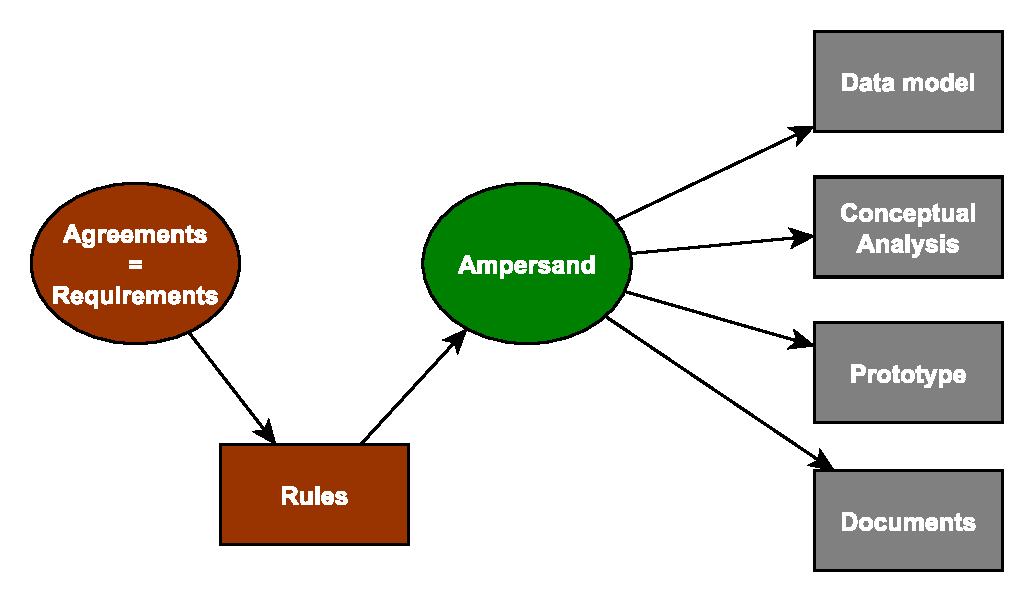
\includegraphics[width=0.7\textwidth]{Figures/Generation}
	\caption[Generated artifacts]{The Ampersand approach generates different artifacts based on the business rules}
	\label{fig:generation}
\end{figure}

\subsection{Project architecture and components}
\label{subsec:architecture}
The compiler developed for the Ampersand research project runs in several steps, hence the Ampersand compiler is also divided in several subcomponents:
\dict{P-structure}{The parse-tree generated by the Ampersand parser, used as input for the type checker.}%
\dict{A-structure}{The ADL code generated by the Ampersand type checker, used as input for the calculator component.}%
\dict{ADL-structure}{See A-structure.}%
\dict{F-structure}{The functional structure generated by the Ampersand calculator, used as input for the different output modules.}%
\begin{description}
	\item[Parser:] This component receives the ADL code as input, and parses that code into a parse-tree (also known as P-structure).
	\item[Type checker:] The Ampersand type checker receives a P-structure as input and converts it into a relational algebra format, suitable for manipulation (also known as A-structure or ADL-structure).
		 The semantics of ampersand are expressed in terms of the A-structure.
	\item[Calc:] The Calc component receives an A-structure as input, and manipulates it according to the research rules, generating the functional structure (also known as F-structure).
		The F-structure contains all design artifacts needed to write a specification and generate the output.
	\item[Output components:] All design artifacts present in the F-structure are ready to be rendered.
		Several components use this data structure to generate the wished output.
		The output components currently implemented (and their output formats) are the following: 
		\begin{itemize}
			\item Atlas (HTML interface);
			\item Revert (Haskell source);
			\item Query (prototype generation);
			\item Documentation Generator (Pandoc structure).
		\end{itemize}
\end{description}
%
The complete architecture is depicted in \autoref{fig:architecture}.
The part of this architecture relevant for this project is depicted in \autoref{fig:data-flow}.
%
\begin{figure}[htb]
	\centering
	\includegraphics[width=\textwidth]{Figures/ADL_systeemarchitectuur}
	\caption[Architecture of the project]{Architecture of the project, showing where the parser fits in the Ampersand system}
	\label{fig:architecture}
	\small
	The components in green background are part of the Ampersand compiler.
	Components in orange are part of the Ampersand Prototype compiler.
	Finally, components in white background are future components, not yet implemented.
\end{figure}
%
\begin{figure}[htb]
	\centering
	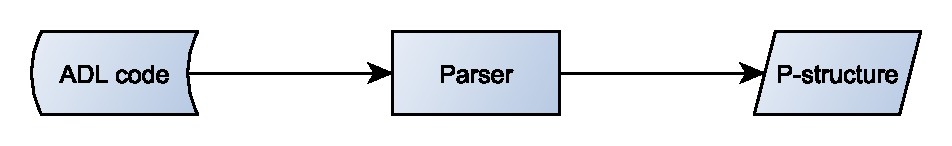
\includegraphics[width=0.5\textwidth]{Figures/Architecture}
	\caption{Relevant data flow for the Ampersand parsing component}
	\label{fig:data-flow}
\end{figure}

\subsection{Current situation}
The end-to-end process of the ampersand project, from compiling towards the generated artifacts, is correct, however there is a major improvement topic identified in the first step, the parsing of the input scripts.

One of the main complaints from users is the quality of the errors generated by the Ampersand parser making it hard for the end users to correct faulty ADL statements.
Since the beginning of the project, the parser subcomponent never received special attention, and it has not been analyzed for improvements.

In order to generate better, useful and to the point error messages, it is assumed that a complete refactoring of the parser will be necessary.
The main challenge is to choose the correct kind of architecture and libraries in order to generate user-friendly messages.

Besides the main project task of improving the parser's feedback, a list of user wishes has accumulated over the years.
The main customer and other users would appreciate if as many wishes as possible could be fulfilled.

\subsection{Goals of the project}
\label{subsec:project-goals}
The main objective for the graduation project is to implement useful feedback in the Ampersand parser.
This will be delivered as  a well-working and maintainable piece of software which needs to be user friendly by which the the usability will be improved.
In order to achieve this goal, the following research \& analysis activities will take place:
\begin{itemize}
	\item Analysis of user-friendly messages in compilers;
	\item Comparison of different Haskell parsing libraries (also for pretty-printing);
\end{itemize}
%
Additionally, the following activities may also take place:
\begin{itemize}
	\item Researching tools and techniques in Haskell for improving the software quality (e.g. testing and error messages);
	\item Analysis of the current development environment in relation with software engineering principles such as continuous delivery/integration;
	\item Recommending improvements for the overall software quality;
\end{itemize}
%
In case the new parser is successfully implemented and accepted, while the project members still have time budget available, the list of open user wishes issues can be addressed.
Some of these wishes are substantial, so that most of them cannot be fulfilled during the graduation project.
The current list of open issues has been provided \cite{open-issues}, although it must be clear that the issues are strictly seen as lower priority.
See also \autoref{sec:requirements} for the list of high-level requirements.

On top of the the project goals, the project members declare herewith to have the following personal objectives and commitments fulfilled by the end of this graduation project:
\begin{description}
	\item[Knowledge:] Building up knowledge is the main reason why one starts a bachelor study.
		As such it is important to learn more about functional programming, Haskell, compilers, business rules and research in general.
	\item[University:] Hopefully the final thesis will be of use for the university and other students.
	\item[Graduation:] As this is a graduation project, it is natural to have the graduation as an important objective.
\end{description}

\subsection{Critical success factors}
\label{subsec:success-factors}
The following factors are critical for the project's successful completion.
Each critical success factor is covered by one or more measures outlined in this project plan:
\begin{description}
	\item[Maintainability:] the code shall at least be as maintainable as the current Ampersand code.
		It is known, however, that maintainability is hard to measure (see also \autoref{sec:risk-management}).
	\item[Production code:] the implemented functionalities shall be integrated into the master branch for production use;
	\item[Users context:] in order to provide useful feedback, the user context wherein the Ampersand compiler is used needs to be well understood, and the improvements must have extra user value. 
		Just like maintainability, useful feedback is a hard to measure topic, this risk is listed in \autoref{sec:risk-management} and will be addressed in phase 3c (research context).
	\item[Communication:] Independent on how good the project results are, if the solution is put into production without proper communication and documentation leading to confused and demotivated users, the project will be perceived as a failure. 
	Although the project aims to add the feedback in the ampersand parser as transparent as possible, the final customer and user perception remains a critical success factor of this project;
\end{description}
%
The syntax of the Ampersand grammar is specified in EBNF notation.
Any changes to the syntax must be documented according with this notation.
The notation can also be added as comment in the source code, in order to make clear that the complete grammar is implemented correctly.

\subsection{Assumptions and constraints}
\label{sec:assumptions-constraints}
The following assumptions and constraints are considered in this project plan:
\begin{itemize}
	\item For the main objectives, the majority of the changes are concentrated in the parser.
		It is assumed that the changes in other parts of the software will be very limited.
	\item The architecture as described by the customer and documented on the Ampersand Wiki is assumed to be correct and up-to-date.
	\item The delivered software will be reviewed and tested by the project team, if the customer needs additional test before the code can be released into the production environment, we assume that the customer will test the new code within one week after project team's tests. Theses specific releases will be communicated well in advance to make sure that the customer can plan these testing activities.
	\item The assumption is made that two project members will be available for an average of 12 hours a week.
		This can be influenced by the members' jobs or private lives.
	\item Regression testing can be done using the available Sentinel Server
	\item Given the major impact on the parser part, we assume that this project team has the lead over the parser code during the project.
		Any fixes are changes on the parser outside the project team will be aligned first on impact and coherence with the ongoing parser changes.
\end{itemize}


% !TEX root = ../Planning.tex
\section{Project approach (M)}
\label{sec:project-approach}
Just like any other project, this project needs a fit-for-use approach. 
This section 'project approach' summarizes the project methodology we will apply together with an exhaustive overview of the project planning, milestones and corresponding deliverables.
\subsection{Project methodology}
The main drivers to determine our project methodology is based on the kind of deliverables that needs to be produced due to this project, more specific, the actual technical realization of the project.

We can group the technical realization into 2 categories:
\begin{enumerate}
	\item The introduction of a new error message approach to provide clear and useful error messages and warnings towards the end-users
	\item Stand-alone modification points toward the Ampersand Parser based on
	\begin{enumerate}
		\item Reported issues
		\item Enhancements
		\item Extensions
	\end {enumerate}
\end {enumerate}

Given the stand-alone aspect of the modification points, the use of an iterative approach is quite obvious as we already have a backlog of topics which can be taken up independently of each other. 

The error messages need somewhat more attention to guarantee that we build up a solid error message architecture. 
The project team will therefore realize a Proof-of-Concept to demonstrate the correct approach and base architecture. 
After validation of this POC, the project team will realize the error message architecture and actual implementation in an iterative approach.
More information on the approach is described in \autoref{sec:project-realization}.

Within this project methodology, following aspects are identified as important to guarantee a qualitative project within time, budget en corresponding to the agreed on project scope : 
\begin{enumerate}
	\item Project management
	\item Knowledge acquisition 
	\item Project realization approach
	\item Integration \& release
	\item Testing \& validation
	\item Communication
	\item Documentation
\end {enumerate}

All these approach topics are fully documented within this project plan.


\subsection{Project phases}
 \begin{enumerate}
	\item Phase 2 - Task allocation and Project plan
	todo: description of phase
	\item Phase 3a - Domains \& Techniques
	todo: description of phase
 	\item Phase 3b - Investigation context (todo: find good translation for 'Onderzoekscontext)
	todo: description of phase
 	\item Phase 3c - Design \& implementation
	todo: description of phase
 	\item Phase 3d - Project documentation
	todo: description of phase
	\item Phase 4 - Project closure and final project presentation	todo: description of phase
\end {enumerate}

\subsection{Project planning, milestones and corresponding deliverables }
The project is planned based on the project milestones and the detailed project planning. The milestone will be formalized by the delivery of their corresponding deliverables

A commitment is given by the project team to adhere to the following milestone planning, officiated by the delivery their corresponding deliverables, grouped by their corresponding project phase:

 \begin{enumerate}
	\item Phase 2 - Task allocation and Project plan
 	\begin{enumerate}
		\item Delivery of the detailed project plan 			- 	13/11/2014
		\item Detailed allocation of tasks within the project team 	- 	13/11/2014
	\end {enumerate}
	\item Phase 3a - Domains \& Techniques
 	\begin{enumerate}
		\item Delivery of scientific article by Daniel			- 	03/12/2014
		\item Delivery of scientific article by Maarten  			- 	03/12/2014
	\end {enumerate}
 	\item Phase 3b - Investigation context (todo: find good translation for 'Onderzoekscontext)
 	\begin{enumerate}
		\item Detailed report of the 'investigation context)  		- 	29/04/2014
	\end {enumerate}
 	\item Phase 3c - Design \& implementation
 	\begin{enumerate}
		\item Analysis \& design documents  				- 	30/03/2014
		\item Test report  							- 	20/03/2014
		\item Source code  							- 	27/03/2014
		\item The actual release of the realized product  		- 	20/04/2014
		\item IT documentation  						- 	20/03/2014
		\item User documentation \& user manual  			- 	20/03/2014
	\end {enumerate}
 	\item Phase 3d - Project documentation
 	\begin{enumerate}
		\item Project documentation document				- 	04/05/2014
	\end {enumerate}
	\item Phase 4 - Project closure and final project presentation
 	\begin{enumerate}
		\item Project essay							- 	20/05/2014
		\item Project presentation						- 	date to be jointly determined, final due date 29/05/2014
	\end {enumerate}
\end {enumerate}

The project activities will be managed in a detailed project planning by the project team, and the status will be shared during project alignment meetings.
Deviations, changes and issues within the project plan will be managed by the project team itself, in full openness towards the project stakeholders. 
As long as the changes to the detailed project plan aren't  compromising the milestone plan, the project is considered to be 'in control'. 

Any deviation of the project plan (due to risks, delays, issues,...) that can have an impact on the project milestone planning will be reported even before they really hit the project plan. 
This way, all project stakeholders will be informed and can cooperate in the corrective actions.





% !TEX root = ../Planning.tex
\section{Project management (M)}
\label{sec:project-management}
This sections descirbes the project management approach and used techniques to gyuarantee project succes.
As the project team consists only out of 2 team members, special attention is given to make the project management approach holistic but light.
Holistic to assure that all important aspects with regards to the management of this project are properly covered and lightweight to avoid that the project team loses time in handling unnecessary tasks which only have added value in larger project teams.
\subsection{Project governance / roles \& responsibilities}
We distinguish 5 different project parties in the project environment:
\begin{enumerate}
	\item The project team
	The project team consists out of Daniel Schiavini and Maarten Baertsoen.
	This team takes the full responsibility for the actual delivery for all project work products consisting out of
	\begin{enumerate}
		\item The actual Haskell program code in full conformity with the coding conventions
		\item Exhaustive code documentation
		\item All necessary final and intermediate deliverables to ensure project success such as: project planning and, project methodology as described within this document. 
	\end {enumerate}
	The full list of all work products with their corresponding description is included in this document.
	\item The project supervisor
	The project supervisor is the main contact person for the project team. It is the role of the project supervisor to monitor the project team on a regular basis as well as to provide support and guidance to the project team members both on content and approach.
	It is the responsibility of the project team to send project status updates towards the project supervisor; these status updates will form the basis for the regular alignment meetings. 
	During project execution, it might occur that the effort needed to meet the customer expectations is way over the foreseen budget of the project, measured in hours. 
	Should this situation occur, the supervisor will facilitate customer alignments to adjust the customer’s requirements.
	All efforts spent are therefore reported on a weekly basis to the supervisor who will track the spent effort to make sure that every aspect of the project receives the needed attention.

	\item The customer
	The project will deliver an actual product with all corresponding documentations in a controlled way. 
	The customer's satisfaction is one of the key success factors of this project.

	Although this project is conducted in a educatinal environment, the customer will be treated just like he would be served in a professional environment. 
	\item End-Users
	The Ampersand Parser is currently used by several users groups 
	\item The examiner

\end {enumerate}


\subsection{Communication}
\lipsum[1]

\subsubsection{Internal}
\lipsum[1]

\subsubsection{OU}
\lipsum[1]

\subsubsection{Customer}
\lipsum[1]

\subsection{Time keeping}
\lipsum[1]

\subsection{Project reporting}
\lipsum[1]

\subsection{Quality assurance}
\lipsum[1]

\subsubsection{Process quality \& monitoring}
\lipsum[1]

\subsubsection{Deliverables quality \& monitoring}
\lipsum[1]

% !TEX root = ../Planning.tex
\section{High-level requirements (D)}
\label{sec:requirements}
\lipsum[1]
% !TEX root = ../Planning.tex

\section{Knowledge acquisition (D/M)}
\label{sec:knowledge-acquisition}

\subsection{Research context (D)}
Some ideas by Bastiaan:
\begin{itemize}
  \item more info on ampersand users
  \item user-friendly error messages (specific to compilers or not)
  \item parser-libraries
  \item Stef's research (3a)
  \item Haskell parsers (e.g. Helium), monadit or combinators
\end{itemize}

\subsection{Domain \& technology}
\subsubsection{Part Daniel (D)}
\lipsum[1]

\subsubsection{Part Maarten (M)}
\lipsum[1]

\subsection{Knowledge documentation (-)}
\lipsum[1]

% !TEX root = ../Planning.tex
\section{Project realization (-)}
\label{sec:project-realization}
\subsection{Coding conventions}
\lipsum[1]
\subsection{Scrum approach}
\lipsum[1]
\subsection{Validation}
\lipsum[1]
% !TEX root = ../Planning.tex

\section{Integration \& release}
\label{sec:integration-release}
\dict{branching}{Branching is the duplication of an object under revision control so that modifications can happen in parallel along both branches.}%
\dict{merging}{The reintegration of a branch into the original code}%
The code changes of this project will be done in a separate branch (\texttt{ABI\_Parser}) of the Ampersand GitHub repository (\texttt{AmpersandTarski/ampersand}).
In the end of each sprint, the project members will evaluate whether the integration into the master branch is advised.
If so, the following steps will be taken:
\begin{enumerate}
	\item The code has already been merged and tested in the project branch.
	\item The project manager shall send a notification via e-mail to the customer, including the test documentation and any other applicable information, such as the commit identifier (see \autoref{subsec:test-documentation}).
	\item The customer should realize any complementary tests and accept the release.
	\item When the release is accepted, a push request will be issued.
\end{enumerate}
%
It is important to note that any code developed in a sprint should be usable and integrated into the master branch.
If integration is not possible, the sprint can be considered failed.
% !TEX root = ../Planning.tex
\section{Risk management (M)}
\label{sec:risk-management}
Risk management is one of the measure taken within the project to guarantee the process quality and hence project success.

The risk management approach consist out of 5 steps

\begin{enumerate}
	\item Risk identification 
	\item Risk qualification
	\item Determine risk mitigation and risk avoidance measures
	\item Monitor and control
	\item Evaluate and fine-tune
\end {enumerate}
\subsection{Risk identification }
Every identified risk within the full life cycle of the project will be listed. A risk is considered every event that can influence the project in a negative way. 
All risks will be kept together in a central repository, the risk register, in which a summary with the main characteristics is provided.
The following information is registered for each risk:

\begin{enumerate}
	\item Risk ID
	\item Status
	\item Domain
	\item Identification date
	\item Short description
	\item Additional information
	\item Mitigation actions
	\item responsible
	\item date next review
	\item Impact
	\item Probability
	\item Risk evolution (status quo, increased or decreased probability)
\end {enumerate}

\subsection{Risk qualification }
Not every identified risk will have the same importance and we will only focus on the risk which are worth our attention.
This means that we will focus on the heavy risks which, if they occur, will have a very bad or catastrophic effect on he project and those that havce a fair chance of occuring but will still have quite a negative impact.


The exact qualification of the risks we will actively manage is based on the risks probability, what is the chance of the risk to becoma a fact, and the risk impact, how hard will this risk impact our project if it happens.

Following matrix identifies the risks qualification based on these 2 parameters:


\begin{table}[h]
\centering
\begin{tabular}{lccc}
Impact & \multicolumn{3}{l}{Likelihood}                                                     \\
       & \multicolumn{1}{l}{Low}   & \multicolumn{1}{l}{Medium} & \multicolumn{1}{l}{High}  \\
High   & \cellcolor[HTML]{FFCB2F}M & \cellcolor[HTML]{FE0000}H  & \cellcolor[HTML]{FE0000}H \\
Medium & \cellcolor[HTML]{34FF34}L & \cellcolor[HTML]{FFCB2F}M  & \cellcolor[HTML]{FE0000}H \\
Low    & \cellcolor[HTML]{34FF34}L & \cellcolor[HTML]{34FF34}L  & \cellcolor[HTML]{FFC702}M
\end{tabular}
\end{table}

Based on the identified risk qualification, the risk will be managed accordingmy:
\begin{enumerate}
	\item L - Low Risk
	Low risks will be monitored on a regular basis, but no speciifc actions will be initiated with regards to risk mitigation and risk avoidance.
	\item M - Medium Risk
	Medium risk wil be managed in a more pro-active way, possible risk mitigation options will be documented and will be taken into account for during the riks life cycle. It is up to the project team to see if the risk is managed actively or if tis will be merely monitored.
	\item H-High risks
	The project team will act on high sense of urgency. High risks will be investigated in detail, a risk mitigation approach will be installed and the risk will be monitored intensively throughout the risk life cycle.
\end {enumerate}
 

\subsubsection{Determine risk mitigation and risk avoidance measures}
The possible risk management strategies used to cope with each distinct risk are the following:
\begin{enumerate}
	\item Risk avoidance
	Actions are undertaken to avoid the risk, meaning that the risk will dissapear due to 
	\item Risk Reduction
	The risk itself cannot be avoided, but measures are taken to limit the negatvive consuquences in case the risk materilases.
	\item Risk sharing
	This kind of risks cannot be coped with by the project team on tits own, therefore the risk is shared with other team to identify a joint risk approach.
	\item Risk acceptance
	The project teams decides to just accept the risk, identifies the risk impact and foresee time and budget to handle with the negative consequences once the risk has materilzes.
\end {enumerate}

The risk management strategy will be documented in the risk register.

\subsubsection{Functional risks}
\lipsum[1]
\subsubsection{Technical risks}
\lipsum[1]
\subsection{Risk mitigation plan}
\lipsum[1]

\subsection{Interferences with other projects}
\lipsum[1]
% !TEX root = ../Planning.tex

\section{Issue management (D)}
\label{sec:issue-management}

% !TEX root = ../Planning.tex

\section{Documentation (R-D)}
\label{sec:documentation}
\subsection{Documentation plan}
Just like the project itself, the documentation will be managed as an iterative product.
All project documentation templates, forming the basis for the documentation deliverables, will be created before the start of phase 3b, investigation context, and all analysis, design and coding documentation will be maintained on a weekly basis.

Each sprint delivery, the available set of documentation will be delivered informally towards the project supervisor and, where useful, towards the client.
The project team strives to finalize all intermediate documentation at least one week after the release corresponding deliverable.

\subsection{Documentation deliverables}
All documentation deliverables, listed in section `Project planning, milestones and corresponding deliverables', are explained in some more detail in this section.

\subsubsection{Detailed project plan}
The detailed project plan, this document, covers at least the following topics:

	\begin{enumerate}
		\item Project description, context and goals
		\item Project approach and project management
		\item Planning
		\item Risks and risk management approach
		\item Quality approach and control
		\item Project requirements, global architecture and the main component, including the environment, of the to be modified system
		\item Test plan
		\item Used tools, methodologies and documentation
		\item knowledge gathering for proper project execution
		\item Communication plan
		\item Glossary
	\end {enumerate}

\subsubsection{Detailed allocation of tasks within the project team}
This project will be driven by 2 project team members who will work closely together.
Based on the personal selection of the  academic competencies, some highlights, responsibilities and corresponding roles will be assigned to each individual team member.

This document will clarify the assigned roles and tasks each team member will take care of.

The `detailed allocation of tasks within the project team' is integrated in the deliverable `Detailed project plan'.

\subsubsection{Scientific article}
Each individual project team member will deliver an in depth analysis of one or more topics regarding the environment in which the system is, or will be, used.

This deliverable will cover at least the following topics:

	\begin{enumerate}
		\item Problem definition
		\item Motivation
		\item Context
		\item Used analysis techniques
		\item Results
		\item Conclusions
		\item Glossary
		\item Bibliography
		\item Appendices, if useful
	\end {enumerate}

\subsubsection{Detailed report of the `investigation context'}
The detailed report of the `investigation context' will cover at least following topics:

	\begin{enumerate}
		\item Context
		\item Conclusions of the researcher
		\item Conclusions in regards to the project
		\item Glossary
		\item Bibliography
		\item Appendices, if useful
	\end {enumerate}

\subsubsection{Analysis \& design}
The `analysis \& design document' will cover at least following topics:

	\begin{enumerate}
		\item Design decisions and the reasoning behind them
		\item Detailed solution design
		\item Implementation guidelines \& coding conventions
		\item Tools \& libraries used in the project
	\end {enumerate}

\subsubsection{Test report}
The `Test report' will cover at least the following topics:

	\begin{enumerate}
		\item Overview of test scenario's
		\item Test results
		\item Conclusions
	\end {enumerate}

\subsubsection{Source code}
The source code will be document in the code itself.
It is of utmost importance that the code is documented in a clear and concise way.
Topics needing a more elaborated documentation approach are documented in the deliverable IT documentation.

\subsubsection{IT documentation}
Some coding structures, or the architectural design principles behind it, can require some additional documentation which could pollute the source code itself.
The IT documentation deliverable will list all complex coding structures and the clarification of them including the overall technical architecture, in accordance with the project scope, and the technical design principles.

The IT documentation must provide the necessary support to our customer to fully understand the project coding and it needs to present a solid basis on which future design and implementation decisions can be taken.

\subsubsection{Project documentation document}
The project will be concluded in a general project documentation document.
This deliverable will conclude all main deliverables, where possible, in a brief way.

Following additional topics will be documented to close the project:
	\begin{enumerate}
		\item Main realizations
		\item Encountered issues \& risks
		\item Tools \& methodologies effectiveness
		\item Topics not delivered with the project
		\item Budget analysis
		\item Lessons learned
		\item Conclusions
	\end {enumerate}
% !TEX root = ../Planning.tex
\section{Tools, methodologies and accelerators}
\label{sec:tools-methodologies}

\subsection{Collaboration}
\dict{Dropbox}{File hosting service that offers cloud storage, file synchronization, personal cloud, and client software}%
\dict{Git}{A distributed revision control and source code management}%
\dict{GitHub}{Git repository web-based hosting service which offers all of the distributed revision control and source code management (SCM) functionality of Git}%
\dict{Microsoft Office}{Office suite of desktop applications developed by Microsoft}%
For the collaboration between the project members, the following tools will be used:
\begin{description}
	\item[Dropbox] For sharing time tracking and other reference documents;
	\item[GitHub] For sharing git repositories of code, besides managing issues and documentation;
	\item[SourceForge] For managing existing issues with the customer and other developers;
	\item[Microsoft Office] For writing internal documents, e.g. time tracking;
\end{description}

\subsection{Documentation}
\dict{Haddock}{A software documentation generator for the Haskell programming language}%
\dict{TeXworks}{Graphical user interface for editing and compiling \LaTeX{} documents}%
\dict{LaTeX}{Document preparation system and document markup language for the TeX typeset}%
\dict{RDG}{Railroad Diagram Generator}%
\dict{Railroad Diagram Generator}{Tool for generating syntax diagrams based on EBNF notation}%
\dict{EBNF}{Extended Backus-Naur Form}%
\dict{Extended Backus-Naur Form}{Notation technique for documenting context-free grammars}%
For writing the documentation, the following tools will be used:
\begin{description}
	\item[Haddock] For annotating documentation on the code;
	\item[TeXworks] For writing, editing and compiling \LaTeX{} documents;
	\item[Ampersand Wiki] For keeping notes and information useful for users and other developers;
	\item[Railroad Diagram Generator] For generating syntax diagrams based on EBNF notation.
\end{description}

\subsection{Design}
\dict{yEd}{Software for editing graphs}%
For designing the software and its architecture, the following tools will be used:
\begin{description}
	\item[yEd] For creating diagrams and graphs;
\end{description}

\subsection{Development}
\dict{IDE}{Integrated Development Environment}%
\dict{GHC}{Glasgow Haskell Compilation system}%
\dict{Cabal}{Library for managing Haskell builds and packages}%
For software development, the following tools will be used:
\begin{description}
	\item[IDE] No standard integrated development environment will be chosen: the project members are free to use any IDE, e.g. Eclipse, Leksah, Notepad++;
	\item[GHC] The compiler GHC (Glasgow Haskell Compilation System), version 7.8.3, will be used;
	\item[Cabal] For managing Haskell packages and compilation, cabal-install version 1.18.0.5 and Cabal library version 1.18.1.3.
\end{description}

\subsection{Testing}
\dict{Hpc}{Library for checking, recording and displaying code coverage}%
\dict{Sentinel}{Test server for the Ampersand project}%
\dict{QuickCheck}{Library for testing Haskell code}%
\dict{HLint}{Library that reads Haskell programs and suggests changes that hopefully make them easier to read}%
Finally, the following tools may be used, where appropriate, for testing the software:
\begin{description}
	\item[Hpc] may be used for checking, recording and displaying the code coverage of tests;
	\item[Sentinel server] can be used for the integration tests;
	\item[QuickCheck] for automating tests on the code and property based testing (e.g. pretty-print and reparsing, random code generation);
	\item[Neil Mitchell's HLint] for checks on the code readability and maintainability;
\end{description}

\newpage
\appendix
% !TEX root = ../ResearchContext.tex

\small
\printglossary[style=mcolindex,title=Glossary]
\label{sec:glossary}

\clearpage
% !TEX root = ../Planning.tex
\addcontentsline{toc}{section}{References}
\label{sec:bibliography}

\begin{thebibliography}{99}

%TODO: Check the order of the bibliography

\bibitem{business-rules}
	The Business Rules Manifesto\\
	Version 2.0, November 1, 2003\\
	Ronald G. Ross\\
	\url{http://www.businessrulesgroup.org/brmanifesto.htm}
	
\bibitem{ampersand-approach}
	Ampersand: foutvrije specificaties voor B\&I-vraagstukken\\
	Informatie magazine, August 2007\\
	Stef Joosten, Rieks Joosten and Sebastiaan Joosten\\
	\url{http://informatie.nl/Artikelen/2007/augustus/Default.aspx}  % AmpersandfoutvrijespecificatiesvoorBI-vraagstukken.aspx
	
\bibitem{ampersand-architecture}
	Ampersand Software Architecture\\
	\url{http://wiki.tarski.nl/index.php/Software_Architecture}
	
\bibitem{pmi}
	Project Management Institute\\
	\url{http://www.pmi.org}
	
\bibitem{open-issues}
	Requirements for a parser of Ampersand\\
	Stef Joosten\\
	Version \texttt{8e27daf}, September 25, 2014\\
%	{\footnotesize \url{https://github.com/AmpersandTarski/ampersand/tree/ABI\_Parser/ArchitectureAndDesign}}
	\url{https://github.com/AmpersandTarski/ampersand/commit/8e27daf}
	
\bibitem{ampersand-wiki}
	Ampersand Coding Conventions\\
	Stef Joosten \& Han Joosten\\
	Version 4, September 6, 2011\\
	\url{http://wiki.tarski.nl/index.php/Coding\_conventions}.

\bibitem{heeren-error}
	Top Quality Type Error Messages\\
	Bastiaan Heeren\\
	ISBN 90-393-4005-6, September 20, 2005\\
	\url{www.open.ou.nl/bhr/phdthesis}.
	
\bibitem{iso-9126}
	Software Engineering -- Product quality\\
	International Organization for Standardization\\
	ISO/IEC 9126:2001\\
	\url{http://www.iso.org/iso/iso_catalogue/catalogue_tc/catalogue_detail.htm?csnumber=22749}.

\bibitem{jstd-016}
	J-STD-016 Standard for Software Development and Documentation\\
	Annex F.2.4: Contents of the Software Requirements Specification (SRS)\\
	Department of Defense, United States of America\\
	September 1995\\
	ISBN 0-7381-0427-2, SS94377.

\end{thebibliography}

\end{document}